\documentclass{article} % Oder eine andere Dokumentklasse wie report, book, etc.
\usepackage[utf8]{inputenc} % Bestimmt die Eingabe-Kodierung
\usepackage[T1]{fontenc} % Bestimmt die Ausgabe-Kodierung
\usepackage{graphicx}


\begin{document}
	
	\title{Deep Reinforcement Learning Exercise 02}
	\maketitle
	
	Group:
	\begin{itemize}
		\item Marvin Kohnen
		\item Moritz Gehring
		\item Julius Ferber 
		
	\end{itemize}
	\section{Exercise 2.1}
	We implemented the grid as a 5x5 matrix using np.array. We also tried to follow the gym library class, by using the functions \_\_init\_\_, step, reset and render (which we really didnt need in this exercise). 
	\subsection{2.1a}
	We implemented the function state\_value\_iteration\_bellman by looping over all the grid cells and computing the state value according to the bellman equation, while handling the "jumping" of the agent for the special states. 
	The plot shows all the state values over time, as well as the state values at the final iteration, using a colormap. As expected, the cells close to the ones, where a positive reward is given, have a quite high state value, and the ones on the bottom of the grid have low state values, with the worst even being negative. 
	As we can see, the state values converge after 10-20 iterations. As we are using a random policy, the state values cannot change after a couple of iterations, since we are not learning anything. 
	
	\begin{figure}[h!]
		\centering
		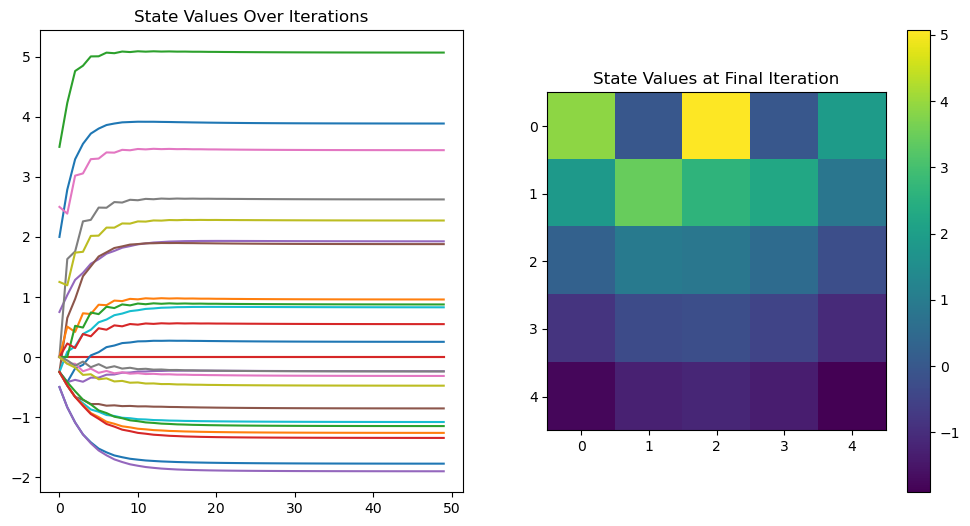
\includegraphics[width=0.9\textwidth]{images/state_values.png}
		\caption{State values over iterations and final iteration}
		\label{fig:2}
	\end{figure}
		
	\newpage
	\subsection{2.1b}
	We implemented the function action\_value\_iteration\_bellman by looping over all grid cells and each action for that grid cell and computing the action value according to the bellman equation. 
	The plots show the action values for all 4 possible directions and each grid cell, as well as all action values over time. Similarily to the first plots, we see high action values for moves onto the cells, which give out the reward, and low action values for the ones moving away from them, with the worst ones also having a negative value.
	
	Again, the action values converge after 10-20 iterations, since the random policy doesn't adjust any actions. 

	The differences between both computations is, that you also have to iterate over all actions, so the number of action values is num\_actions times that of the state values. 
	\newline
	
	\begin{figure}[h!]
		\centering
		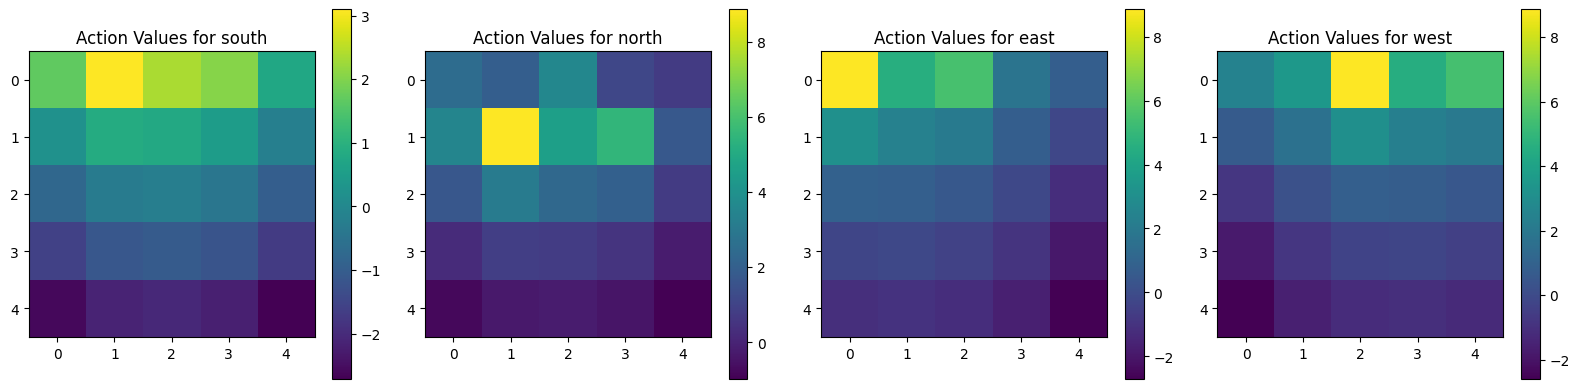
\includegraphics[width=1\textwidth]{images/action_values_per_direction.png}
		\caption{Action values per direction}
		\label{fig:3}
	\end{figure}
	
		\begin{figure}[h!]
		\centering
		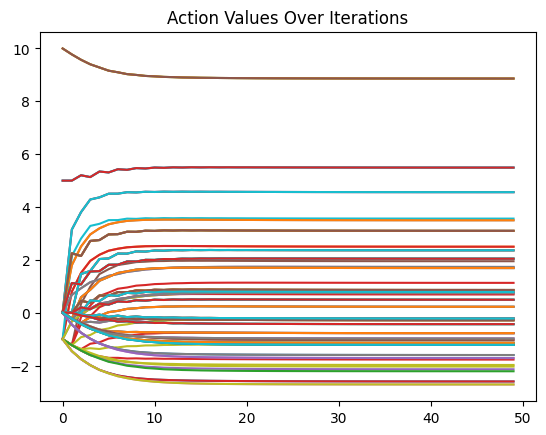
\includegraphics[width=0.9\textwidth]{images/action_values.png}
		\caption{Action Values over iterations}
		\label{fig:4}
	\end{figure}
	
	
	
	
	\section{Exercise 2.2}
	\subsection{2.2.a}
	Nothing much to be said here to be honest. Please note that we kind of failed to understand the urgency of the function "render(mode)". Since it did not hinder the implementation (2.2 b), we did not further investigate but will be delightet to hear about its functionality in the exercise review :D 
	
	EDIT: Nevermind, just read the functionality on the documentation. Would still be nice to see a working example of the "rendering" and its different modes regarding our task.
	
	Furthermore, we discussed what an episode "ending" in this circumstance would entain? It could be the first teleport, n amount of steps or a certain reward threshold (and many more arbitrary events).
	
	\subsection{2.2.b}
	Again, nothing much to be explained. Implementation worked as expected. We can see the "teleport" upon reaching grid space [0,1] in step 12. 
	
	\begin{figure}[h!]
		\centering
		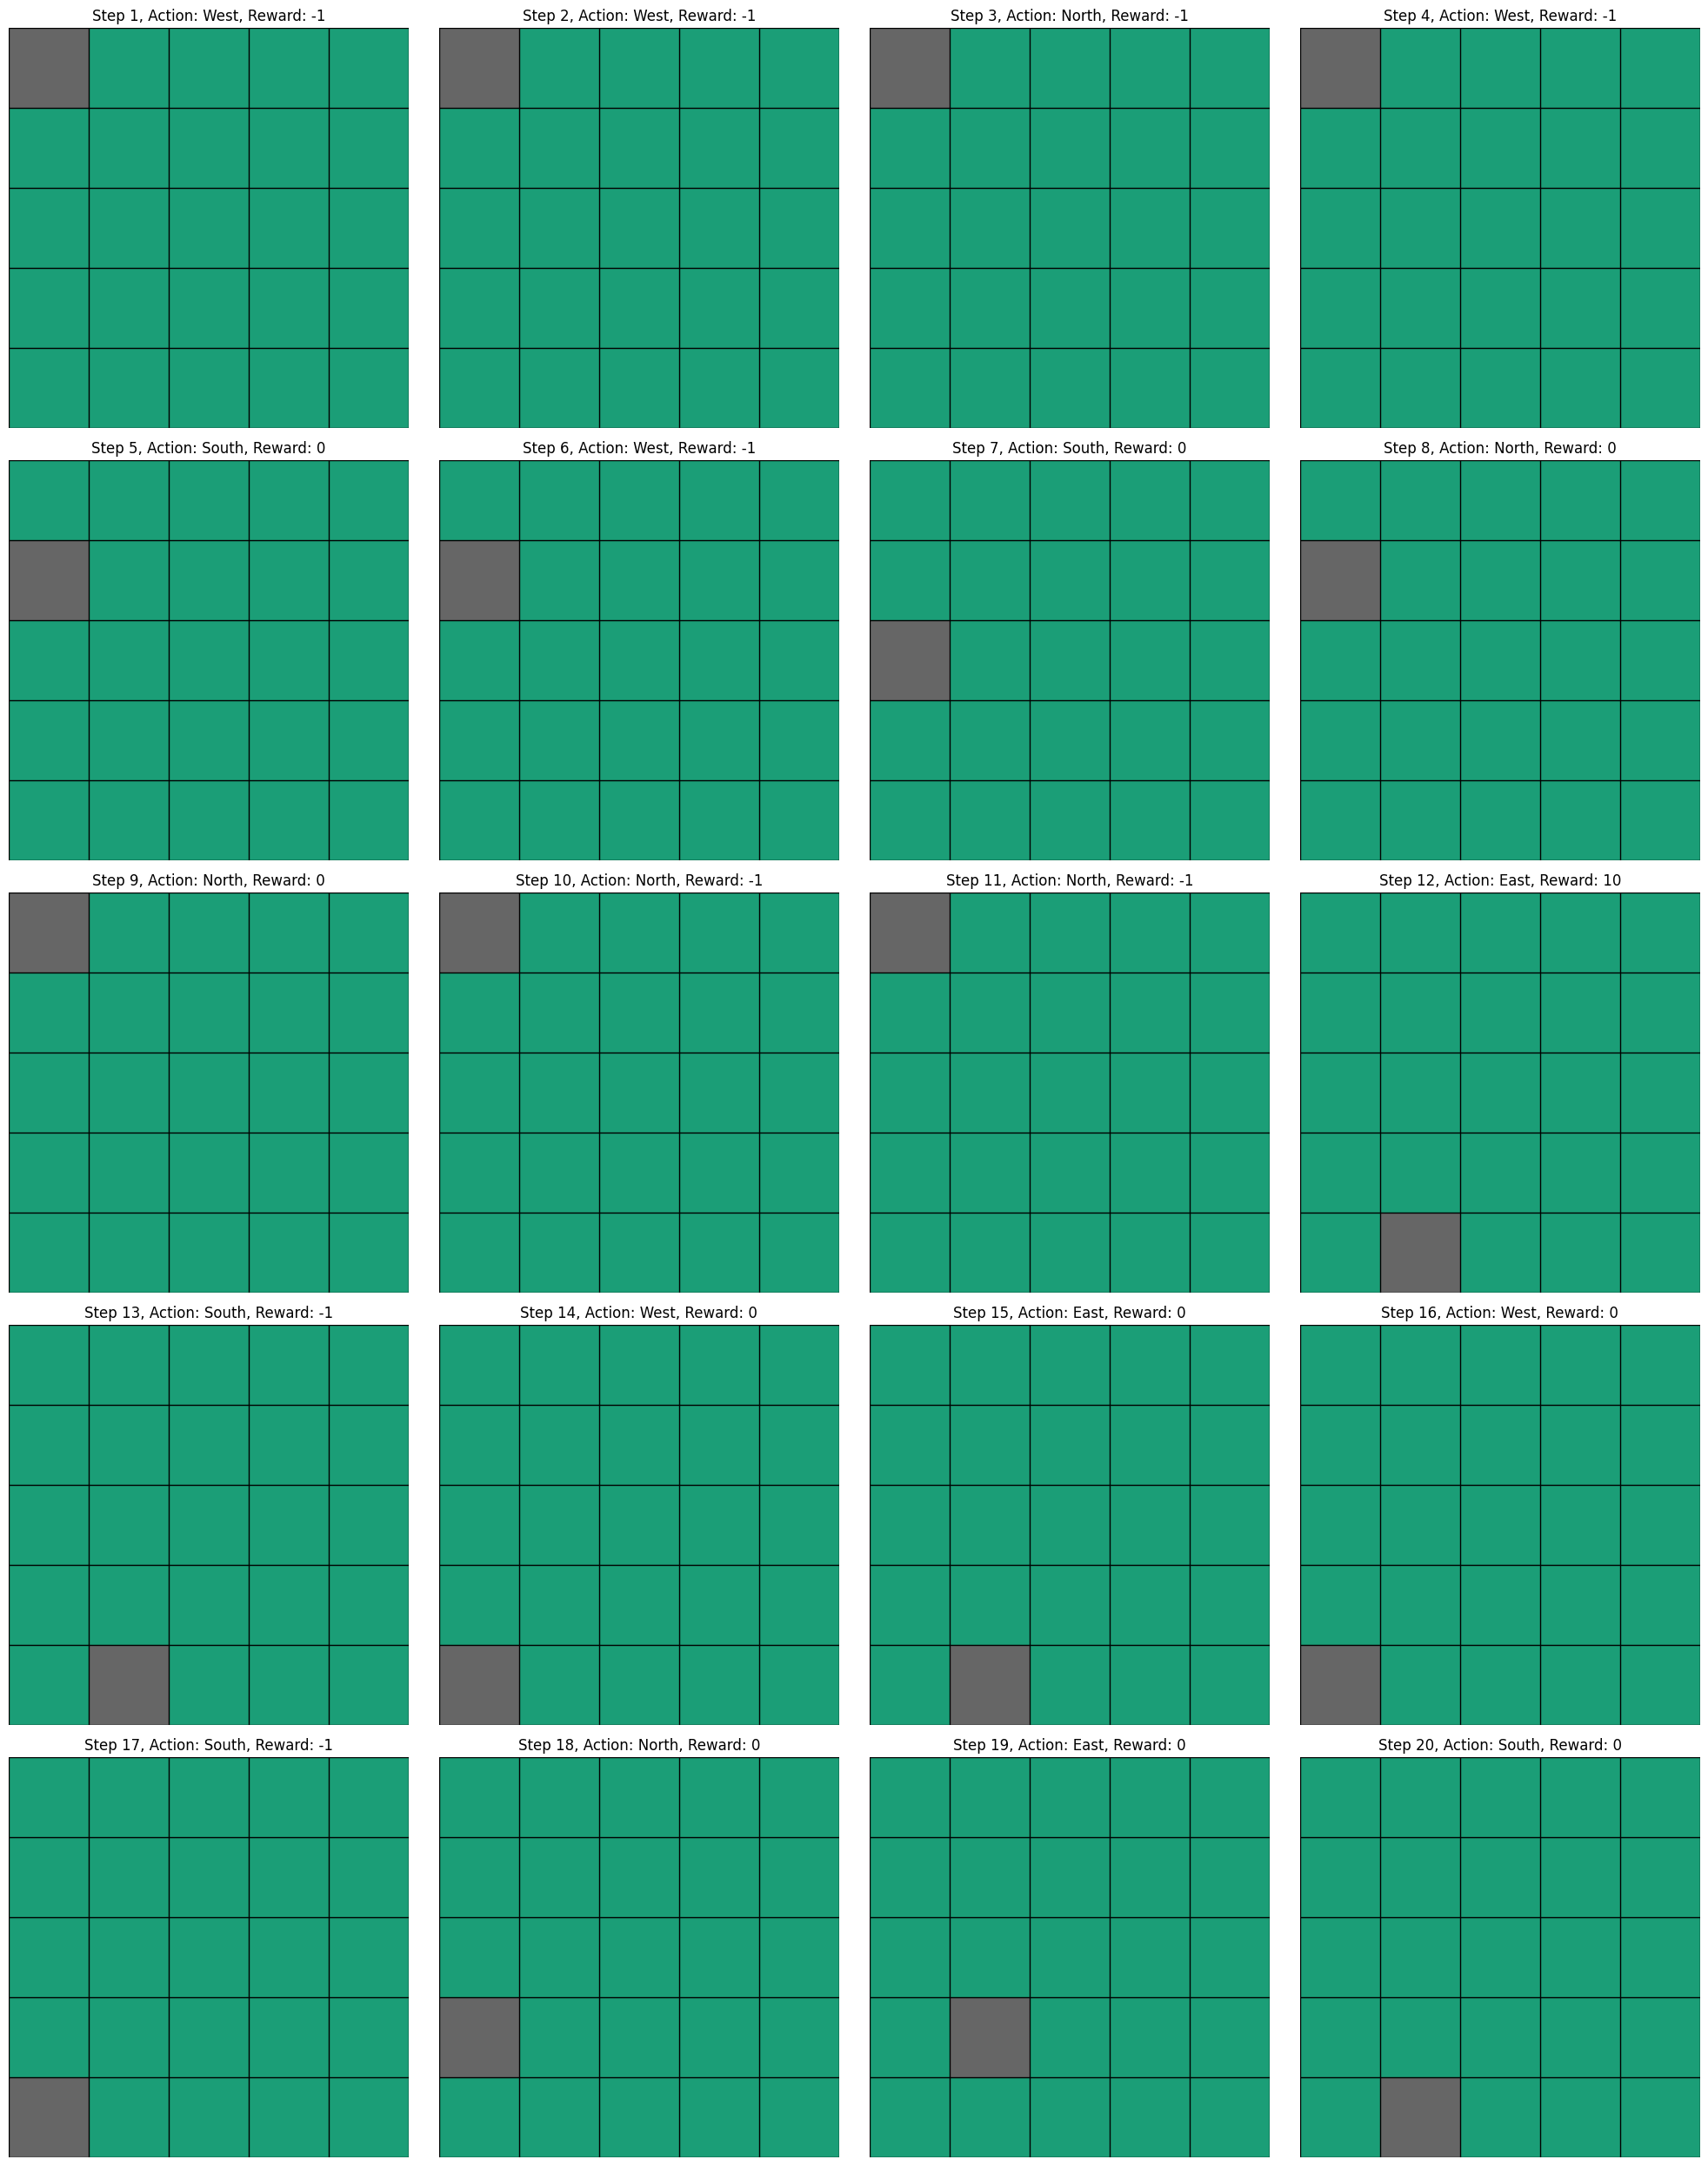
\includegraphics[width=0.9\textwidth]{images/20_steps.png}
		\caption{20 successive steps of the environment}
		\label{fig:1.1.a.1}
	\end{figure}
	
	
	\section{Exercise 2.3}
	\subsection{2.3.a}
	From Documentation: 
	\begin{description}
		\item[State space:] 4 continuous variables:
		\begin{itemize}
			\item Cart Position; Limits: $[-4.8, 4.8]$
			\item Cart Velocity; Limits: $[-\infty, \infty]$
			\item Pole Angle; Limits: $[-24^\circ, 24^\circ]$
			\item Pole Angular Velocity; Limits: $[-\infty, \infty]$
		\end{itemize}
		
		\item[Action space:] 2 discrete actions:
		\begin{itemize}
			\item Push cart to the left
			\item Push cart to the right
		\end{itemize}
		
		\item[Environment dynamics:]
		\begin{itemize}
			\item Start: all variables (Cart Position, Cart Velocity, Pole Angle, Pole Angular Velocity) start with a random value between $-0.05$ and $+0.05$
			\item End:
			\begin{enumerate}
				\item Pole is no longer balanced (angle greater than $\pm12^\circ$)
				\item Cart reaches the edge of the environment (Cart Position greater than $\pm2.4$)
				\item Maximum episode length is met (in this case 500 time steps)
			\end{enumerate}
		\end{itemize}
		
		\item[Reward structure:] 
		\begin{itemize}
			\item Option 1: $+1$ for each time step the pole is balanced
			\item Option 2: $0$ for all time steps, $-1$ when the pole falls (and the episode terminates, see above)
		\end{itemize}
	\end{description}
	
	Simple Simulation of the CartPole environment; 
	code structure taken from gym documentation. The loop chooses a random action at each time step.
	The action is then executed and the environment is rendered. Rendering is delayed by 0.1 seconds after each step,
	as otherwise the simulation terminates after <1 second and cannot actually be observed by humans.
	
	
	
	\subsection{2.3.b}
	It can be clearly seen that the simplest approach, i.e. moving in the opposite direction of the pole's lean is the worst policy. When watching the actual simulation, it can be seen that this very quickly results in overcorrection on the agents part, with the pole oscillating faster and faster, leading to a fall. This is slightly improved by just choosing a random direction when the pole is (nearly) upright. Choosing a random direction is an approach to simulate "doing nothing" in a sense, as the pole is already balanced and no action is required. A significant improvement is achieved when correcting for the angular velocity of the pole, as this directly combats the oscillation and therefore the tendency to overcorrect. 
	Interestingly, it can be seen that ensuring that the cart stays within its positional bounds does not significantly improve the performance of the agent. This is likely to the fact that the cart needs a long time to move to the outer edges, meaning that the case in which the cart reaches the edge is rare and therefore does not significantly impact the overall performance. Lastly, taking the cart velocity into consideration does decrease the agents performance. This is probably because it tends to  unnecessarily change the direction of the cart, which leads to additional angular velocity for the pole, rather than helping to keep it low and the pole upright.
	
	
	\begin{figure}[h!]
		\centering
		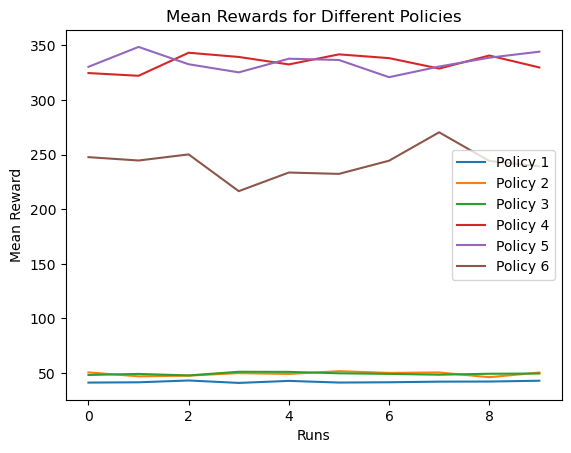
\includegraphics[width=0.9\textwidth]{images/mean_reward.png}
		\caption{20 successive steps of the environment}
		\label{fig:5}
	\end{figure}

	
	\subsection{2.3.c}
	We tried implementing the RL Model, but as you can see in Figure \ref{fig:6} our model does not appear to be learning. Furthermore, our understanding of the "learning process" using 16 distinct bandits for 16 states is not yet fully developed. Therefore we're eagerly waiting for a nice presentation on wednesday :D 
	
	\begin{figure}[h!]
		\centering
		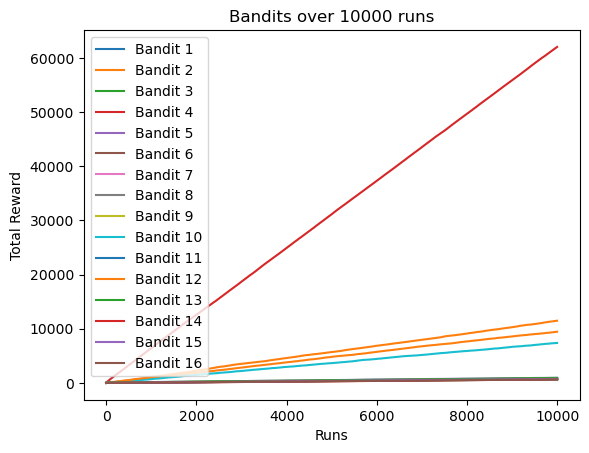
\includegraphics[width=0.9\textwidth]{images/bandits_over_10000_runs.png}
		\caption{Bandit Performance over 10000 runs}
		\label{fig:6}
	\end{figure}
	
	
	\end{document}